\chapter{Konzept}
\label{chap:konzept}

Zur Erstellung des Konzepts gilt es mehrere Aspekte im Voraus genauer zu betrachten.
Dabei wird als erstes in \Cref{sec:weristmeinezielgruppe} die Zielgruppe der Softwarelösung analysiert. Daraufhin
wird in \Cref{sec:anforderungsanalyse} die Anforderungsanalyse der vier Aspekte; Gestaltung, Funktionalität,
Flexibilität und Codebasis behandelt. Nach der Anforderungsanalyse gilt es
in \Cref{sec:auswertungvorhandenersoftwareloesungen} die aktuelle Lage
des Marktes zu analysieren. Tools im Bereich der Geschäftsanalytik gibt es viele. \cite{WikiBISoftware}
Was zeichnet diese Softwarelösungen aus? Mit welchen Merkmalen kann man sich von vorhandenen Lösungen
bewusst unterscheiden? In \Cref{sec:progressivewebapp} und \ref{sec:microservices} beschäftigt
sich die Arbeit mit der Analyse zweier für die Softwarelösung relevanter Technologien.
Bei der ersten Technologie handelt es sich um eine Progressive Web App. Hier gilt es folgende
Fragen zu beantworten: Was ist eine Progressive Web App und macht diese 
im Kontext der Benutzeranforderungen Sinn? Was sind Vor- und Nachteile gegenüber nativer Apps?
Wie sieht es mit der Unterstützung der Plattformen aus? Als zweites wird ein für die
Serverinfrastruktur relevantes Architekturmuster als Lösungsansatz diskutiert. Hierbei
stellen sich folgende Leitfragen: Was versteht man unter Microservices? Was ist der Kompromiss,
den man eingeht, wenn man sich für eine Microservice-Infrastruktur entscheidet?

Sind all diese Fragen beantwortet, kann ein Grundkonzept der Gesamtanwendung entwickelt werden.
Hierbei werden in \Cref{sec:zielsetzung} die Ziele für die Softwarelösung gesetzt. In \Cref{sec:entwurf}
werden daraufhin Entwürfe sowohl von der Benutzeroberfläche als auch von der Infrastruktur vorgestellt.
Weitere Designentscheidungen werden in den folgenden Kapiteln debattiert.

\section{Übersicht}
\label{sec:uebersicht}
In den vorherigen Abschnitten wurden die Anforderungen ermittelt, verwandte Softwarelösungen
studiert sowie zwei relevante Technologien genauer betrachtet. In der Zielsetzung soll nun
anhand der daraus resultierenden Erkenntnisse ein klares, aussagekräftiges Ziel definiert werden.
Dabei müssen Kompromisse eingegangen werden. Aufgabe der Zielsetzung ist es unter anderem,
die Gewichtung auf die zuvor erörterten Anforderungen zu verteilen. In \Cref{sec:entwurf}
wird daraufhin ein grober Entwurf konzipiert. Am Ende der Arbeit wird anhand der Zielsetzung
und der Auswertung ein Fazit gezogen.

Was ist das Ziel dieser Arbeit? Aus rein funktionaler Sicht ist das Ziel dieser Arbeit
folgendes: Eine Webanwendung zu entwickeln, die Daten aus einer API ausließt,
diese verarbeitet und in einem Dashboard veranschaulicht. Nutzer können sich
in der Webanwendung anmelden, externe API-Aufrufe als Datenquellen bestimmen,
die empfangenen Daten verarbeiten, ein Dashboard mit Diagrammen per Drag and Drop erstellen
und den im Dashboard enthaltenen Diagrammen Datenquellen zuweisen. Die erstellten
Dashboards können die Nutzer dann verwenden, um ihre aktuell über die externen 
API-Aufrufe zur Verfügung gestellten Daten auszuwerten. Die Funktionalität
ist das Herz der Anwendung und hat somit aus funktionaler Sicht höchste Priorität.
Aus wissenschaftlicher Sicht ist das Ziel dieser Arbeit die zuvor genannte
Funktionalität mithilfe einer langlebigen, gutdurchdachten, benutzerfreundlichen,
robusten sowie performanten Softwarearchitektur zu verwirklichen. Auf wissenschaftlicher
Ebene spielt die Auseinandersetzung mit der Erforschung und Findung einer möglichst perfekten
Lösung für die Verwirklichung eines solchen Systems, eine, der Implementierung selbst,
übergeordneten Rolle. Dabei stellen sich folgende Fragen: Wie kann ein möglichst agiler
Prozess der Erstellung eines Dashboards aussehen? Wie muss die Logik innerhalb des Systems
getrennt werden? Wie kann der Datenfluss optimiert werden? Wie können Qualitätsmerkmale
gesichert werden? All diese und noch viele weitere Fragen gilt es zu beantworten.

Wie sieht es mit der Gewichtung der in der Anforderungsanalyse in \Cref{sec:anforderungsanalyse}
ausgearbeiteten Anforderungen an die Gestaltung, Funktionalität, Flexibilität und Codebasis aus?
Am einfachsten kann man diese Frage beantworten, in dem man sich klarmacht, was keinen wissenschaftlichen
Mehrwert hätte. Eine API im Frontend aufzurufen, die erhaltenen Daten hartkodiert zu verarbeiten und
in einer möglichst größen Anzahl an hartkodierten Diagrammen anzuzeigen. Das würde eventuell auf den
ersten Blick gut aussehen, hat aber mit der Entwicklung einer soliden Softwarelösung nichts zu tun.
Um eine solide Softwarelösung bewerkstelligen zu können, benötigt es eines soliden Softwaredesigns.
Ein solches Design soll das primäre Ziel dieser Arbeit sein. Robert C. Martin sagt zur Qualität eines
solchen Designs folgendes:
"Die Qualität des Designs bemisst sich schlicht und ergreifend an dem Ausmaß des Aufwands, der
erforderlich ist, um den Bedürfnissen der Kunden gerecht zu werden. Bedarf es hierfür eines
geringen Aufwands und bleibt dies auch während der gesamten Lebenszeit des Systems so,
dann handelt es sich um ein gutes Design — steigt der Aufwand mit jedem neuen Release,
taugt das Design nichts. So einfach ist das."\cite[S. 30]{RobertC.Martin2018} Was heißt
das aber nun für die Gewichtung der in der Anforderungsanalyse erarbeiteten Anforderungen?
Ziel dieser Arbeit ist es bei der Entwicklung der Softwarelösung mehr Wert auf die Flexibilität
der Software als auf den Funktionsumfang einzelner Merkmale zu legen. In unserem
vorherigen Beispiel heißt das konkret: Richtig ist es, eine Software zu entwickeln, die zwar erst ein Diagramm
implementiert hat, wo aber der Vorgang, ein weiteres Diagramm hinzuzufügen, vereinfacht wurde.
Falsch ist es, eine Software zu entwickeln, wo zwar bereits hunderte Diagramme implementiert sind,
der Vorgang, ein neues hinzuzufügen, allerdings immer komplexer wird.

\section{Tests Konzept}
\label{sec:testskonzept}
Um die Anforderungen an die Tests zu erschließen, muss zuerst die Anforderung an die verschiedenen
Arten von Tests gestellt werden. Dabei gibt es verschiedene Sichtweisen.


Zum besseren Verständnis hier ein
paar Beispiele: Tests aus Sicht des Benutzers sind End-To-End-Tests, die User Stories nachahmen.
So kann mit Cypress, einem JavaScript-Framework für End-To-End-Tests, GUI-Interaktionen getestet werden.
Tests aus softwaretechnischer Sicht sind meistens Modul- und Integrationstests. Somit kann die reibungslose
Kommunikation zwischen verschiedenen Teilen der Softwarearchitektur sichergestellt werden. Qualitätsmerkmale
von Webseiten können mit Lighthouse, einem Open-Source Werkzeug von Google, getestet werden. \footnote{https://developers.google.com/web/tools/lighthouse}
Lighthouse testet Performanz, Zugänglichkeit, optimale Vorgehensweisen, SEO und die Unterstützung
des Funktionsumfangs von PWAs.

Wo sind Tests zwingend erforderlich und wo sind sie überflüssig? Um diese Frage zu beantworten, muss
man die Vor- und Nachteile, die Tests mit sich bringen, abwägen. Was sind diese Vor- und Nachteile?
Tests sind von grundaus essentiell für die Qualitätssicherung der Software. Allerdings bringen Sie auch
einen Implementationsaufwand mit sich. Dieser ist bei dem Lösen von komplexen Problem um einiges kleiner
als das Lösen des Problems selbst. Ein testgetriebener Ansatz kann sogar den Lösungsvorgang beschleunigen,
da man sich die benötigte Funktionalität bei der Implementierung der Tests verdeutlicht.
Bei kleinen Problemen ist die Implementierung der Tests allerdings komplexer als das Problem selbst.
Hier können Tests den Entwicklungsvorgang bremsen. Dies trifft speziell auf schnelllebige Teile der 
Software zu. So macht es keinen Sinn, im Frontend eine GUI-Komponente zu testen, bei der man sich nicht sicher ist,
ob man diese nicht innerhalb kürzester Zeit wieder verwürft. In Bezug auf die Anforderung an die Testabdeckung dieser Arbeit bedeutet das;
Im Frontend sollten vorerst nur komplexe Problemstellungen getestet werden. Auf Integrationstests und Tests
zu Qualitätsmerkmalen der Anwendung sollte großer Wert gelegt werden. Um die Softwarequalität kontinuierlich
zu sichern, müssen die Tests in den automatisierten Softwareauslieferungsprozess eingebunden werden. 
So sollte kein Merge auf den Master möglich sein, wenn nicht die CI-Pipeline fehlerfrei durchlaufen wurde.
Zu den zuvor als relevant definierten Testarten gilt die Aussage aus dem Buch Clean Code von Robert C. Martin:
"Die Tests sind solange unzureichend, wie es Bedingungen gibt, die nicht von den Tests geprüft werden,
oder Brechnungen, die nicht validiert werden." \cite[S. 370]{CleanCode}

\section{Flexibilität externer Schnittstellen}
\label{sec:flexibilitaetexternerschnittstellen}
Nun gibt es zwei Optionen.
Erstens: Man entwickelt für jede Änderung der Schnittstelle eine neue Version seiner Software. Zweitens:
Die Information über die Beschaffenheit der Schnittstelle kommt in die Datenbank und nicht in den
Quellcode.

Vergleicht man die zwei im vorherigen Absatz genannten Optionen anhand des Implementierungsaufwandes,
kommt man auf folgendes Resultat: Auf kurze Sicht gewinnt die erste Option. Sie ist einfach zu implementieren.
Man programmiert die benötigten Aufrufe der Datenquellen in der angeforderten Reihenfolge in den Quellcode.
Möglicherweise fehlt noch ein bestimmter Aufruf, also fügt man diesen hinzu.
Option zwei ist um einiges schwerer zu implementieren. So muss man die Beschaffenheit sowie die Reihenfolge der Anfragen
gegen die API in der Datenbank persistieren, diese auslesen und ausführen. Es ist möglich, dass die Daten zwischen den
Anfragen verarbeitet werden müssen. Dieser Lösungsansatz fordert eine durchdachte Softwarearchitektur. Wie sieht es mit den
zwei Optionen auf lange Sicht aus? Option zwei ist mit der Implementierung fertig. Die Softwarearchitektur
benötigt für folgende Änderungen der Schnittstelle nur einen neuen Datenbankeintrag. In Kontrast dazu steht Option eins.
Hier muss für jede Änderung der Schnittstelle der Quellcode angepasst werden. Dies ist ein niemals endender Prozess.
Der Implementierungsaufwand ist also unendlich.

Eins gilt es bei dem zuvor durchgeführten Vergleich allerdings zu beachten. Beide Optionen haben ihre Daseinsberechtigung
und machen je nach Situation auch durchaus Sinn. Es wäre falsch zu sagen, dass eine dieser beiden Optionen die richtige ist. Für einen
Machbarkeitsnachweis \footnote{In der Businesswelt spricht man hier oftmals von einem POC (Proof of Concept).}
ist Option eins eine gültige Lösung. Wenn der Änderungsaufwand im Quellcode sehr gering ausfällt oder sich
die Beschaffenheit der Schnittstelle nur sehr selten ändert, ist Option eins plausibel und eventuell kostengünstiger.
Aufgrund der oben genannte Fakten ist davon auszugehen, dass die Softwarelösung mit unterschiedlichen Schnittstellen arbeiten muss.
Die Beschaffenheit der Schnittstellen kann sich stetig anpassen. Um diese Anforderung an die Flexibilität
der Software bereitzustellen, verfolgt diese Arbeit den Ansatz aus Option zwei.

\section{Trennung der Logik}
\label{sec:trennungderlogik}
Die Benutzerverwaltung muss klar von der Zulieferung der Daten getrennt werden.
In der Zulieferung müssen die Daten verarbeitet und für die Frontendanwendung
vorbereitet werden. Dieser Rechenaufwand ist nicht mit dem der Benutzerverwaltung
zu vergleichen. So kann bei der Datenzulieferung die Menge der über die Netzwerkverbindung
gesendeten Daten stark variieren. Dies ist in der Benutzerverwaltung nicht der Fall. 
Hier werden maximal zehn Ressourcen wie Benutzer, Datenquellen, Dashboards oder Charts
auf einer Seite angezeigt. Die Nutzlast verhält sich somit statisch. Für dieses Verhalten
eignet sich eine REST-API über HTTP. Die Orientierung an den Entitäten spiegelt sich in der Navigation
im Frontend wider. Die Zulieferung der auszuwertenden Daten muss in Echtzeit erfolgen.
Hier ist eine bidirektionale Kommunikation zwischen Server und Client von Vorteil.
Für solch eine Kommunikation eignet sich eine WebSocket-Verbindung. Nach dem über HTTP erfolgten
Handshake rüstet sich die Verbindung auf das WebSocket-Protokoll auf. Die WebSocket-Verbindung
findet direkt auf der TCP-Schicht statt, wodurch man den HTTP-Mehraufwand umgeht.\footnote{Dieser Mehraufwand ist beispielsweise der bei jeder Anfrage mitgeschickte HTTP-Header}
Eine WebSocket-Verbindung ist allerdings serverseitig sehr teuer, da die Verbindung während der Nutzung
der Webanwendung kontinuierlich aufrechterhalten werden muss.\footnote{Man könnte natürlich die Verbindung immer wieder neu öffnen, der dafür nötige Handshake ist allerdings kostenaufwändiger als eine einfache HTTP-Abfrage.} 
Es ist also essentiell, dass der Service, der sich um die Zulieferung der auszuwertenden Daten kümmert,
getrennt von dem, der die Benutzerverwaltung bereitstellt, skaliert werden kann.

Es sollte keine direkte Kommunikation zwischen dem Service der Benutzerverwaltung und dem
Service der Datenzulieferung bestehen (siehe Abbildung \ref{figure:trennungderlogic}).
Jeder Service besitzt sein eigenen Cache und seine eigene Datenbank. Somit sind
die Services komplett unabhängig entwickel-, ausliefer- und skalierbar. Die Abhängigkeit der einzelnen
Services mit dem Frontend ist natürlich immernoch gegen. Diese Abhängigkeit muss man
allerdings in Kauf nehmen.

Der Benutzerverwaltungsdienst sowie der Datenzulieferungsdienst sind als einzelne Microservices
im Backend zu verstehen. Ziel ist es, diese Services in Zukunft durch weitere Services zu ergängen.

\begin{figure}
    \begin{center}
    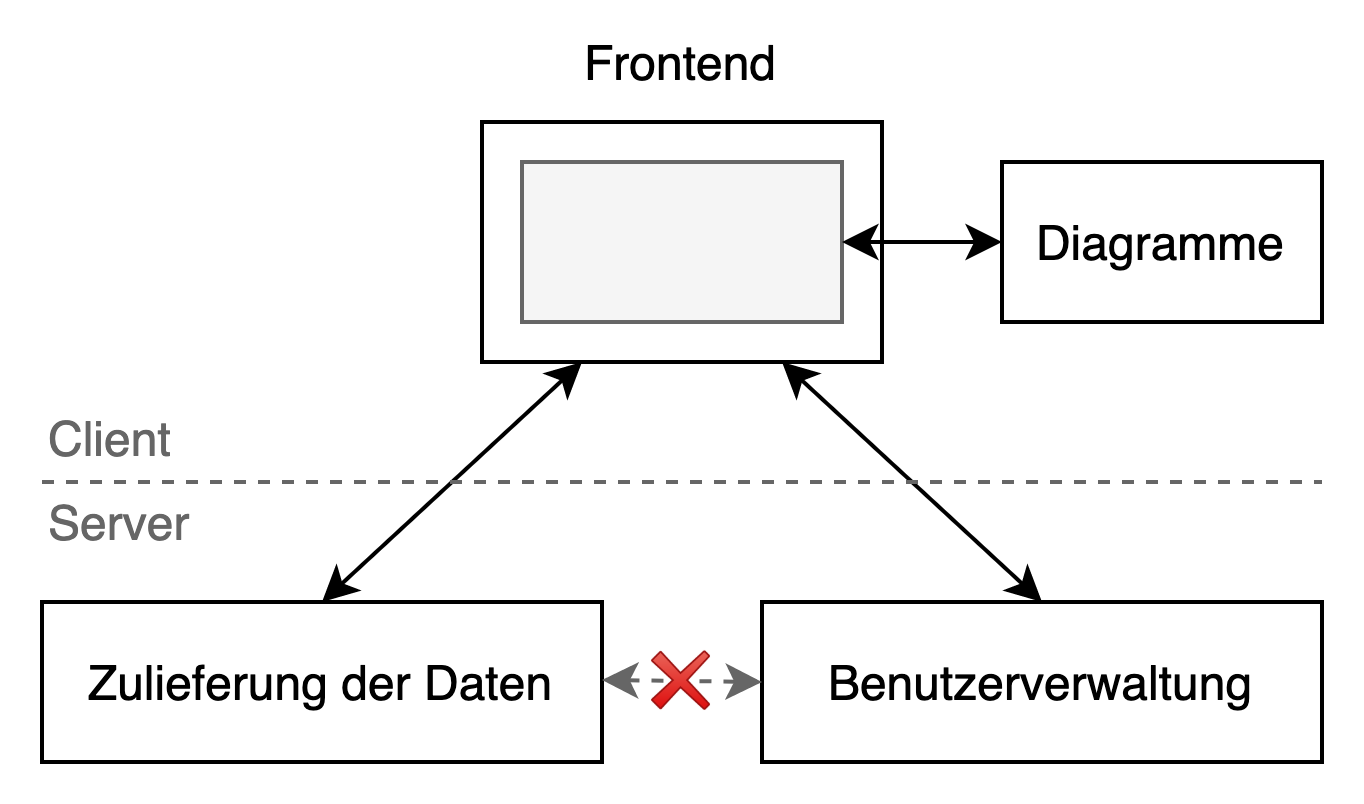
\includegraphics[scale=0.2]{img/abbildungen/TrennungDerLogic}
    \end{center}
    \caption{Trennung der Logic}
    \label{figure:trennungderlogic}
\end{figure}

Die Arbeit verfolgt auch für das Frontend einen Microservice-Ansatz. Man spricht hier von einem
Microfrontend. Michael Geers schreibt dazu in einem Artikel auf Digital Pioneers folgendes:
"Der Ansatz, der sich jetzt förmlich aufdrängt, ist die Umsetzung der Microservice-Idee
auch im Frontend. Anstatt einer ­großen Single-Page-Applikation baut man mehrere unabhängige
Teilapplikationen, die miteinander kommunizieren. Diese sind dann deutlich einfacher zu verstehen.
Der Einsatz einer neuen Technologie lässt sich in einem kleineren Rahmen testen."\cite{MicrofrontendT3N}
Dabei sollen die Diagramme eines Dashboards als einzelne Services ausgelagert werden (wie in Abbildung \ref{figure:trennungderlogic} dargetstellt).
Die Diagramme können so einzeln entwickelt und ausgeliefert werden. Aufgrund der
gleichen Machenschaft der Schnittstellen der Diagramme, kann man diese Art des Code-Splittings auch als
einen Plugin-Ansatz ansehen. Die Diagramme sollen über die In-Memory-Datenbank
Redis zur Verfügung gestellt werden. Die PWA selbst soll vorerst über einen
Nginx Webserver und später über ein CDN ausgeliefert werden. Die Diagramme werden mithilfe
von Dynamic Imports\footnote{Dynamic Imports gibt es seit ES6 (ECMAScript 2015)\cite{DynamicImportsV8}}
während der Laufzeit agil nachgeladen. Da immer nur die verwendeten Diagramme aus der In-Memory-Datenbank
geladen werden, kann die Webanwendung eine nahezu unendliche Auswahl an möglichen Diagrammen zur Visualisierung
der Daten bereitstellen.

\section{Strategie der vereinten Frontendanwendung}
\label{sec:vereintefrontendanwendung}

\section{Monorepo und Git-Submodules}
\label{sec:monorepoundsubmodules}
In diesem Abschnitt geht es um die Aufteilung des
Programmcodes in Repositories. Für die Versionsverwaltung
wird Git verwendet. Die Arbeit entscheidet sich dazu,
die einzelnen Microservices in einer Monorepo unterzubringen.
Unter Monorepo versteht man die Strategie, den Programmcode
aus mehreren Anwendungen, Services, Bibliotheken und Frameworks
in einer Repository unterzubringen.\cite{MonorepoTrunkBasedDevelopment}
Diese Strategie verringert nicht nur den Aufwand
des Aufsetzens mehrerer Repositories, sondern gibt den
Entwicklern auch einen besseren Überblick über die einzelnen
Projekte. Gerade im Fall von Microservices hat dieser
Ansatz den Vorteil, dass man Änderungen in mehreren Services,
die miteinander verkoppelt sind, in einem Commit in die
Versionsverwaltung einchecken kann. Dies kann verbindlich sein,
wenn Tests der Pipeline auf bestimmte Versionen der unterschiedlichen
Services angewiesen sind. Verändert man beispielsweise
eine API eines Services, kann man gleichzeitig das Frontend
anpassen. Die Diagramme eines Dashboards sollen allerdings
auch extern entwickelbar sein. Um dies zu ermöglichen, verwendet
die Arbeit Git-Submodules.\cite{GitsubmodulesGitSCM} Mithilfe dieser Submodules
kann man andere Repositories in ein Repository integrieren. Somit können externe Entwickler das Repository des
Submodules gabeln\footnote{Unter "gabeln" oder auch "forken" versteht man
das Erstellen einer eigenen Kopie eines Repositories, mit der unabhängig von
der Versionierung der gegabelten Repository entwickelt werden kann.},
um in ihrem eigenen Repository Diagramme für die Anwendung zu entwickeln.
